\section{Physarum Polycephalum}
\label{section:background_physarum}

The organism being a subject for this work is \textit{Physarum Polycephalum} also called the many-headed slime mould. It is a member of the \textit{Physaridae} family of slime moulds, in order of \textit{Physarales}, class \textit{Myxogastria}, phylum \textit{Myxomycete}, supergroup \textit{Amoebozoa} in \textit{Protista} kingdom. While current position in taxology is well defined, presented characteristics will justify why scientists used to have problems with classification of the Physarum \cite{stephenson1994myxomycetes}.

In order to make the thesis readable, terms \textit{Physarum Polycephalum}, \textit{Physarum} or \textit{the slime mould} will be used interchangeably as the subject is unambiguously defined. 


\subsection{Biological characteristics}

\textit{Physarum Polycephalum} is a very peculiar organism. Even being a \textit{Protista} it can be observed with a naked eye --- it holds a record for the biggest living unicellular ogranism \cite{TODO}. 

\begin{figure}
  \centering
  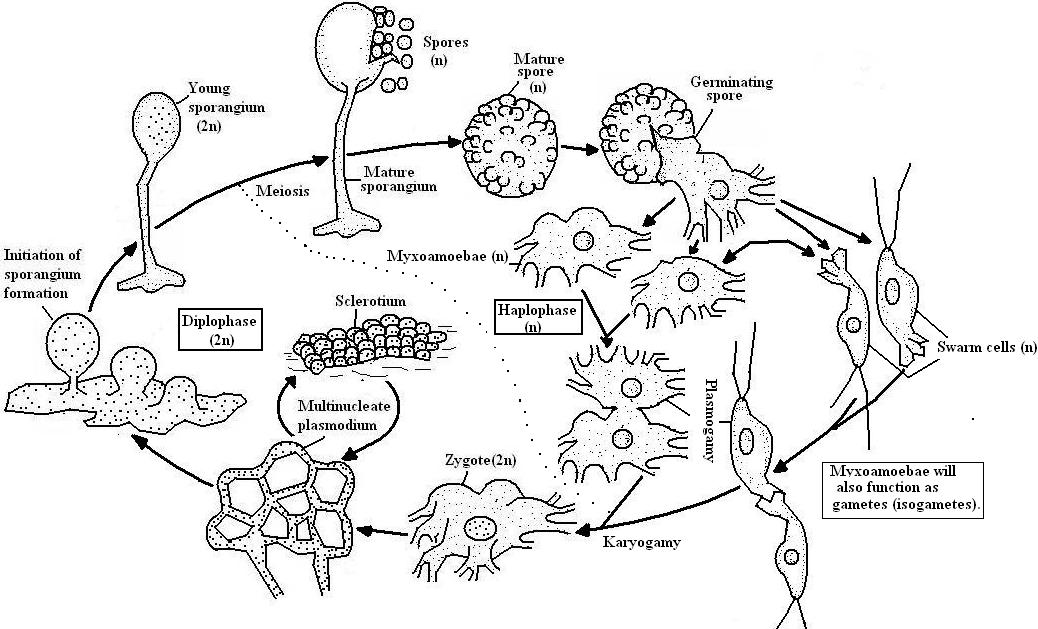
\includegraphics[width=0.94\textwidth]{background/physarum/lifecycle.png}
  \caption{Lifecycle of \textit{Physarum Polycephalum} \cite{TODO}}
  \label{figure:bp_lifecycle}
\end{figure}

As representant of \textit{Myxomycete}, a life cycle of the slime mould is very complex (as seen in figure \ref{figure:bp_lifecycle}). For purposes of unconventional computing applications, \textit{Physarum} is preferred in its plasmodial stage. However, during research transformations into other states are inevitable and must be dealt with.


\subsection{Observations}

lorem


\subsection{Emerging computational possibilities}

lorem


\subsection{Interaction}

lorem

